\subsubsection{Simplificação dos modelos genéricos e parametrização dos cenários}
\noindent A simulação energética e análise de um único cenário requer a utilização da ferramenta básica de modelagem, construção e revisão, que neste caso foi a ferramenta \textit{OpenStudio}. Entretanto, como este trabalho analisa vários cenários pertinentes a mais do que um modelo, foi necessária uma ferramenta mais robusta, que proporcionasse simulações simultâneas dos cenários construídos. Para esta finalidade, a ferramenta de parametrização PAT foi utilizada.\vspace*{0.3cm} \newline
\noindent Entretanto, um requisito necessário para que as simulações ocorram de forma simultânea e consumam pouco tempo de recurso computacional é a simplificação dos modelos. Esta simplificação consiste em reduzir o número de zonas térmicas a serem simuladas por meio da subtração de pavimentos que não sofrem influência da radiação solar e intempéries em uma edificação.\vspace*{0.3cm} \newline
\noindent Diante do exposto, o primeiro e o ultimo pavimento, juntamente ao pavimento intermediário a eles, foram mantidos, como apresentado na Figura \ref{fig:figure20}. Este recurso de redução de tempo de simulação é possível utilizando a função multiply disponibilizado pelo \textit{EnergyPlus} \cite{U.S.DepartmentofEnergy-USDOE2019}. Esta função tem como característica replicar os pavimentos selecionados a fim de multiplicar o número de zonas térmicas, área de piso e energia consumida pela carga interna virtualmente, substituindo as zonas térmicas modeladas e excluídas anteriormente.\newline
\begin{figure}[H]
    \caption{Modelos genéricos simplificados.}
    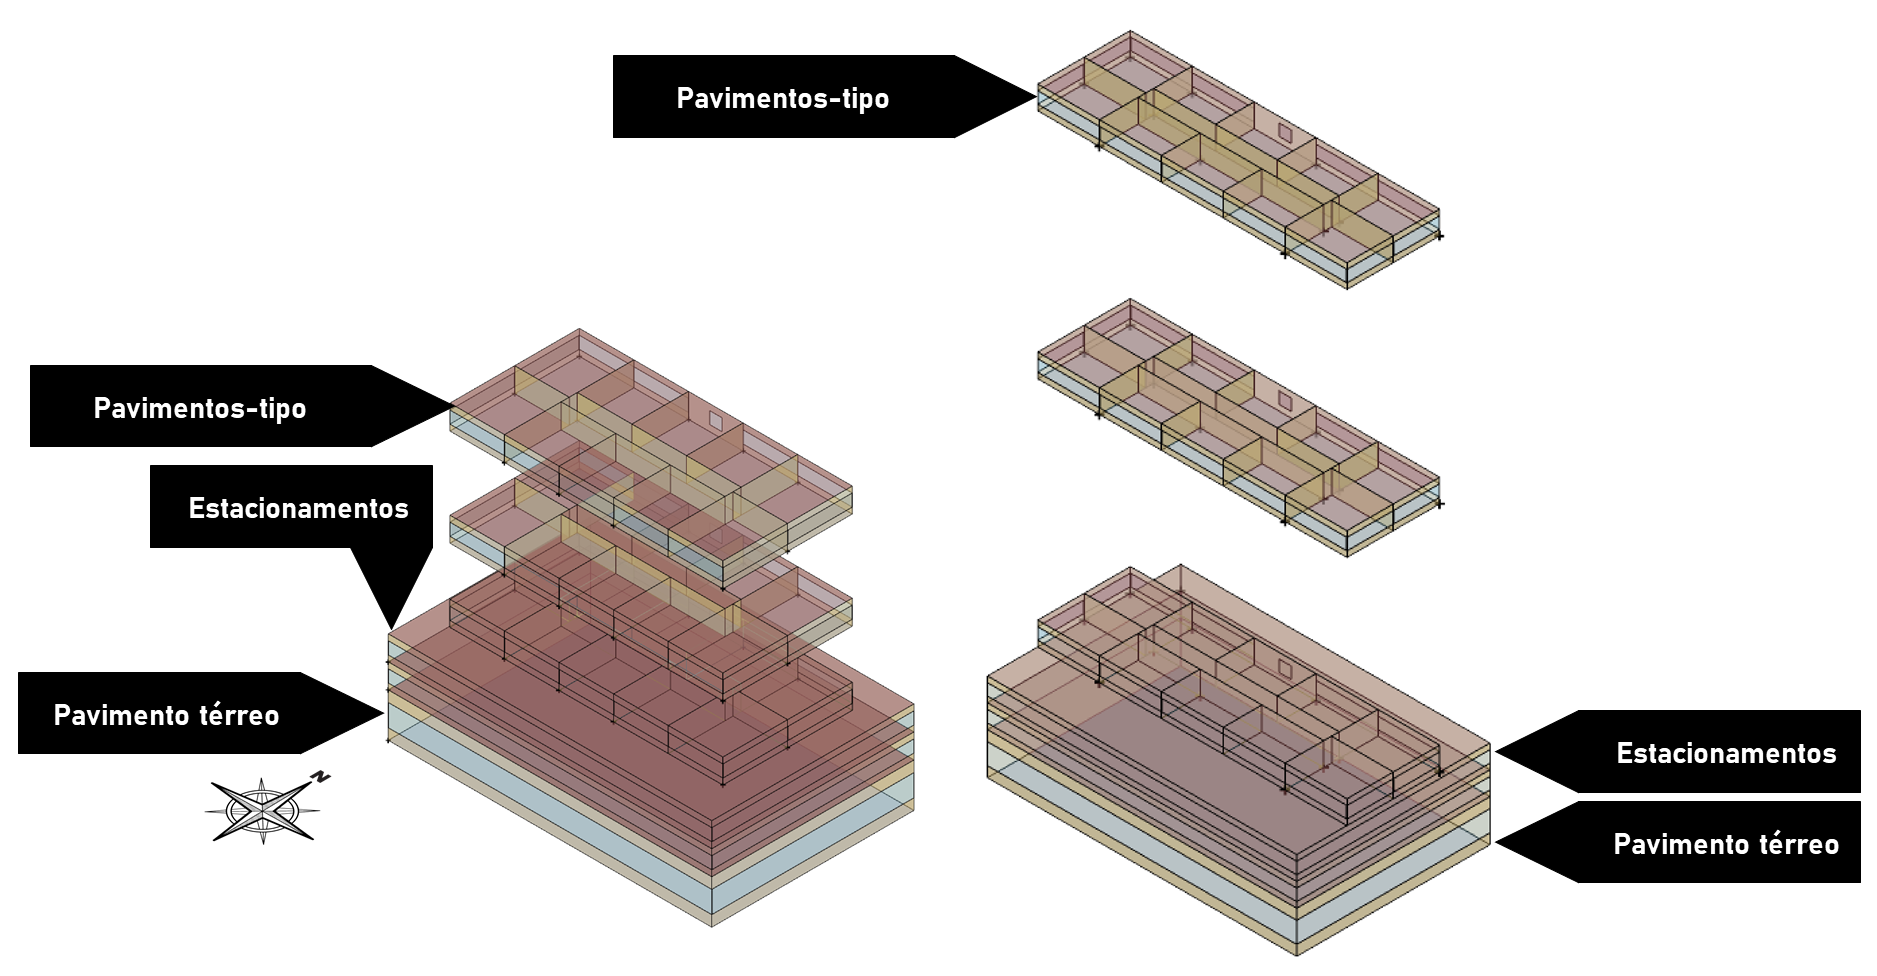
\includegraphics[width=1.0\textwidth]{figures/fig20-modelos.png}
    \begin{flushleft}
        \par \small Fonte: autor, (2019).
    \end{flushleft}
    \label{fig:figure20}
\end{figure}
\noindent Assim, a partir dos modelos simplificados, foram configurados os 368 cenários utilizando a ferramenta PAT, processo ilustrado pela Figura \ref{fig:figure21}. Desta forma, estes cenários que abrangem a etapa de otimização dos modelos genéricos foram simulados simultaneamente, reduzindo o tempo total de simulação e obtenção de resultados.\newline
\begin{figure}[H]
    \caption{Interface do \textit{Parametric Analysis Tool.}}
    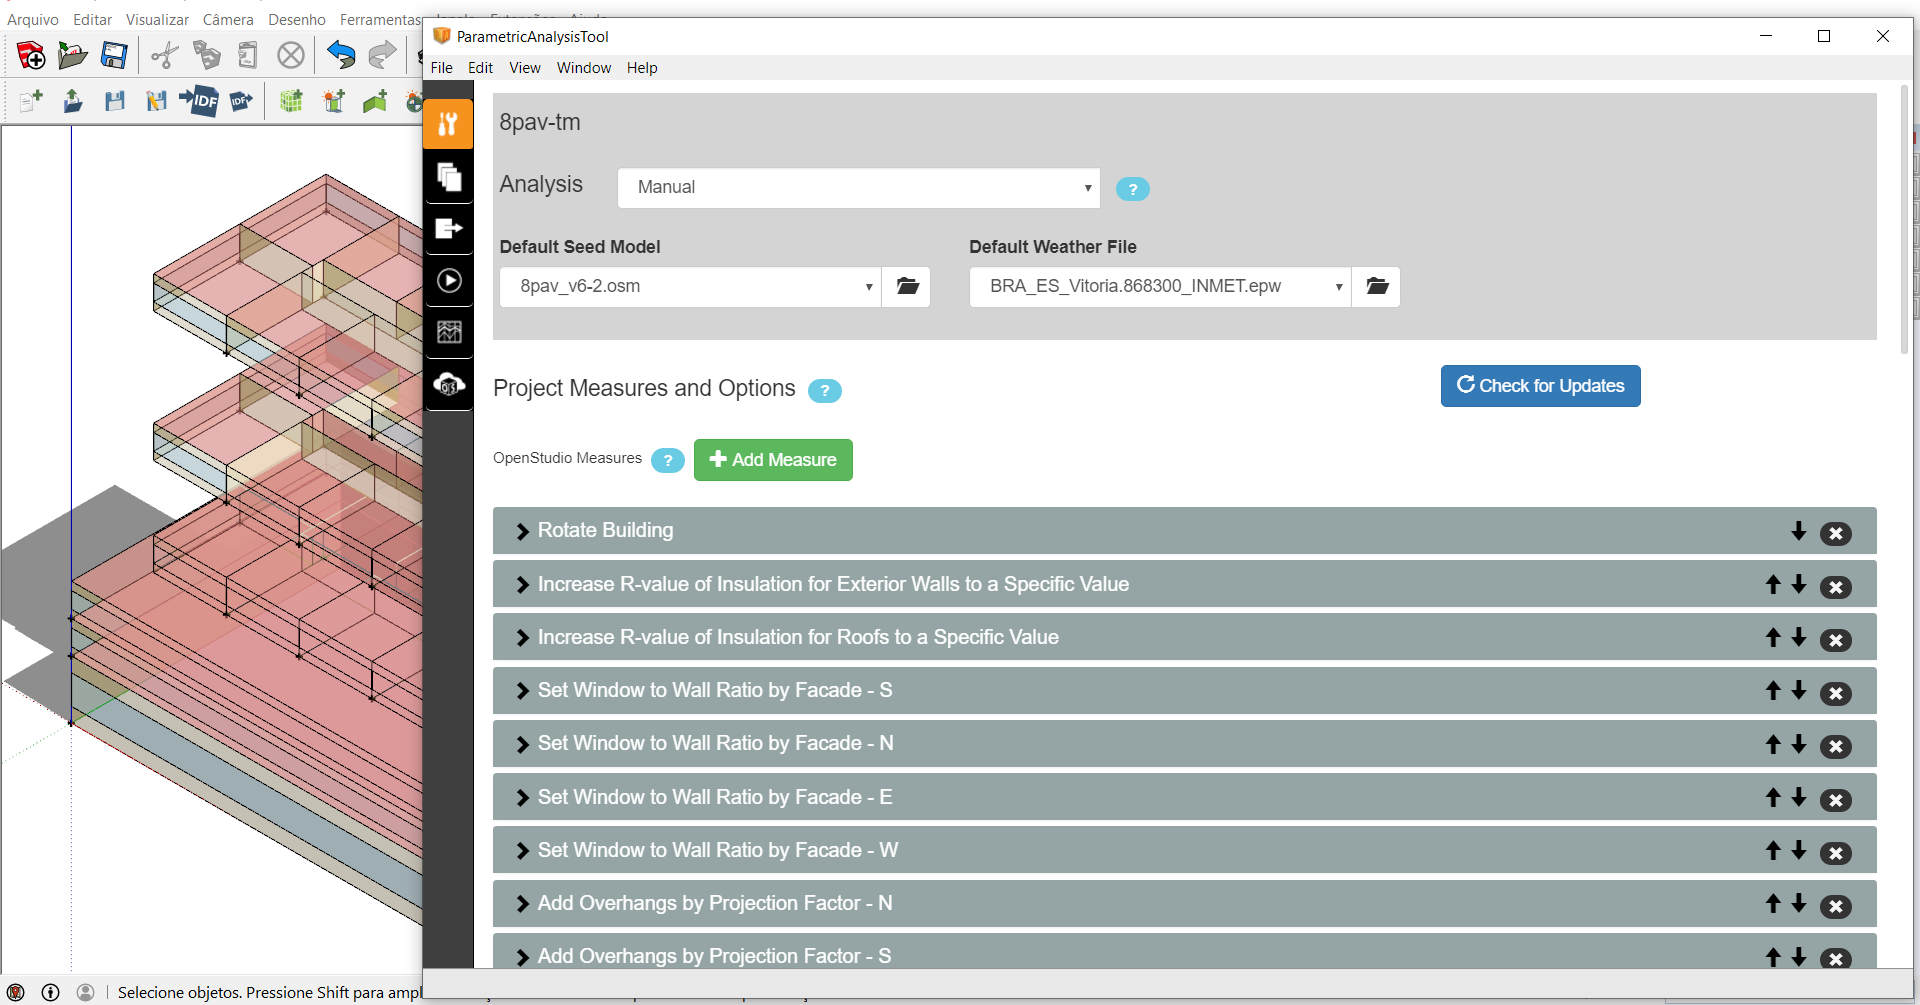
\includegraphics[width=1.0\textwidth]{figures/fig21-modelos.png}
    \begin{flushleft}
        \par \small Fonte: autor, (2019).
    \end{flushleft}
    \label{fig:figure21}
\end{figure}
\subsubsection{Processo de modelagem}
\noindent A partir da etapa de otimização, as informações reunidas sobre as estratégias passivas e ativas utilizadas neste trabalho serviram como base de dados para a configuração das measures no processo de simulações da PAT. As measures de estratégias ativas, como as medidas substituição do sistema de condicionamento de ar e de redução de carga de energia elétrica, foram executadas, respectivamente, no primeiro e no último bloco de simulações, compreendendo as reduções ativas de Intensidade de Uso de Energia e consumo final energético.\vspace*{0.3cm} \newline
\noindent Concomitantemente, os blocos de simulação implementados entre as medidas ativas de redução de energia englobaram as estratégias passivas, como mudança de PAF\textsubscript{T}, de componentes construtivos e alterações volumétricas e de orientação solar das fachadas. O processo de simulação dos cenários obedeceu a sequência de implementação das medidas para redução de consumo de energia disposta na Tabela \ref{tab:tabela13}.\vspace*{-0.1cm}
\begin{table}[H]
    \small
    \caption{\textit{Measures} utilizadas e os parâmetros correlacionados.}
    \begin{tabular}{llll}
    \hline
    \multicolumn{1}{c}{\textit{\textbf{Measure}}}                                                                                        & \multicolumn{1}{c}{\textbf{Parâmetro alvo}}                                                       & \multicolumn{2}{c}{\textbf{Inputs}}  \\ \hline
    \multirow{3}{*}{\makecell[l]{\textit{ZEGD VRF with DOAS;} \\ \textit{Add aPSZ-HP to each zone}}}                            & \multirow{3}{*}{\makecell[l]{Sistema de Condicionamento \\de Ar}}                                                 & a  & \textit{CAG/Fancoil}            \\
                                                                                                                                &                                                                                                   & b  & \textit{Split}                  \\
                                                                                                                                &                                                                                                   & c  & VRF                             \\ \hline
    \multicolumn{1}{l}{\multirow{4}{*}{\textit{Rotate Building}}}                                                               & \multicolumn{1}{l}{\multirow{4}{*}{Orientação solar}}                                             & a  & 0°                              \\
    \multicolumn{1}{l}{}                                                                                                        & \multicolumn{1}{l}{}                                                                              & b  & 90°                             \\
    \multicolumn{1}{l}{}                                                                                                        & \multicolumn{1}{l}{}                                                                              & c  & 180°                            \\
    \multicolumn{1}{l}{}                                                                                                        & \multicolumn{1}{l}{}                                                                              & d  & 270°                            \\ \hline
    \multirow{3}{*}{\makecell[l]{\textit{Increase R-value of Insulation for} \\ \textit{Exterior Walls to a Specific Value}}}   & \multirow{3}{*}{\makecell[l]{Transmitância térmica \\da parede da envoltória}}                    & a  & 2,46 W/m²K                      \\
                                                                                                                                &                                                                                                   & b  & 0,38 W/m²K                      \\
                                                                                                                                &                                                                                                   & c  & 0,32 W/m²K                      \\ \hline
    \multirow{3}{*}{\makecell[l]{\textit{Increase R-value of Insulation for} \\ \textit{Roofs to a Specific Value}}}            & \multirow{3}{*}{\makecell[l]{Transmitância térmica da \\cobertura}}                                               & a  & 3,73 W/m²K                      \\
                                                                                                                                &                                                                                                   & b  & 0,55 W/m²K                      \\
                                                                                                                                &                                                                                                   & c  & 0,53 W/m²K                      \\ \hline
    \multirow{3}{*}{\textit{Set Window to Wall Ratio by Facade}}                                                                & \multirow{3}{*}{\makecell[l]{Percentual de Área de \\Abertura da Fachada Total}}                  & a  & 30\%                            \\
                                                                                                                                &                                                                                                   & b  & 50\%                            \\
                                                                                                                                &                                                                                                   & c  & 80\%                            \\ \hline
    \multirow{3}{*}{\textit{Add overhangs by Projection Factor}}                                                                & \multirow{3}{*}{Proteção solar}                                                                   & a  & 20 cm                           \\
                                                                                                                                &                                                                                                   & b  & 50 cm                           \\
                                                                                                                                &                                                                                                   & c  & 100 cm                          \\ \hline
    \multirow{2}{*}{\textit{Reduce Lighting Loads by Percentage}}                                                               & \multirow{2}{*}{\makecell[l]{Medidas de Redução de Carga\\ de Energia Elétrica: Iluminação}}      & a  & n/a                             \\
                                                                                                                                &                                                                                                   & b  & 30\%                            \\ \hline
    \multirow{2}{*}{\textit{Reduce Equipment Loads by Percentage}}                                                              & \multirow{2}{*}{\makecell[l]{Medidas de Redução de Carga\\ de Energia Elétrica: Equipamentos}}    & a  & n/a                             \\
                                                                                                                                &                                                                                                   & b  & 30\%                            \\ \hline
    \multirow{2}{*}{\textit{Add, Remove or Replace Window}}                                                                     & \multirow{2}{*}{\makecell[l]{Vidros com transmitância \\térmica baixa}}                                           & a  & 0,44 W/m²K                      \\
                                                                                                                                &                                                                                                   & b  & 0,16 W/m²K                      \\ \hline
    \end{tabular}
    \begin{flushleft}
        \par \small Fonte: autor (2019).
    \end{flushleft}
    \label{tab:tabela13}
\end{table}
\vspace{-0.60cm} \noindent Com estas medidas, buscou-se atingir a eficiência energética necessária para o balanço energético dos modelos propostos, complementando a economia com produção de energia de fontes renováveis.
